\chapter{Introduction}\label{chapter_introduction}
% Describe the research domain
% - scope: networked embedded systems, safety-critical, real-time, distributed
% - interesting problems:
Networked embedded systems are prevalent today in many safety-critical domains, e.g., automotive systems, avionics, industrial automation, etc., and are expected to increase their share in the automation of safety critical applications. They are characterized by stringent timing and reliability requirements in order to perform correctly, thus guarantee safe system operations. Moreover, they are usually run on resource constrained hardware platforms, e.g., with limited power supply, memory and CPU which demand more efficient software development \cite{es} as compared to traditional software systems, e.g., web and desktop software applications. A typical example of such systems is a brake-by-wire system, which is an active safety feature in modern automotive cars that have replaced mechanical braking by software and electrical capability \cite{ref}. It runs a distributed embedded software application on a single or multiple computation nodes (or computing units) also known as electrical computing unit (ECU), and has stringent high-level timing constraints, e.g., on the duration of braking the vehicle to the desired level, as well as timing constraints at the subsystem levels. Due to the constrained nature of the electrical/electronic architecture of vehicles, the brake-by-wire systems is developed with awareness especially on critical system resources, e.g., power and energy consumption, computation and communication resources, such as CPU and memory. Therefore, safety-critical embedded systems are expected handle functional complexity while at the same time satisfy timing constraints, as well as performance and quality standards in order to provide better solutions and thus be competitive in the market.

% Describe challenges
% - challenges: 
% - existing solution:
% - what is lacking
Over the last decades, the complexity of networked embedded systems has increased rapidly, that is more and more functions (or software applications) running on limited hardware platforms, for instance, as compare to 2000, the number of software applications running on electrical/electronic vehicle architecture have increased by x, and likewise, the number of lines of code increased by x. To this effect, several development paradigms and computational architectures are introduced and assessed. In the former case, model-based development has been applied successfully to cope the complexity of software and system development, e.g., on requirements modeling, design and implementation, verification and validation, and deployment, that is by providing different abstraction of the system with appropriate modeling languages, e.g., generic architectural languages such as UML, SysML, domain-specific architectural languages, such as AUTOSAR, EAST-ADL in automotive domain, functional behavioral modeling languages, e.g., Simulink, Modelica, etc. In the latter case, many architectures have moved from federated to distributed architecture, and even to consolidation of safety-critical and non-critical software application on common execution platform, e.g., with the mixed-critical deployment of avionics distributed software applications. However, the lack of rigorous analysis support and efficient computation platform is still an impediment to the correctness of complex safety-critical embedded systems. In particular, the lack of effective and robust, yet scalable methods and tools for the specification of software and system requirements and verification of system models against such specifications is a stumbling block in achieving dependable safety-critical systems especially for practical (or industrial) problems, as such capability reduce software errors at the early stages of development and thus reduce maintenance cost, and improve product quality and competitiveness. Moreover, the deployment of distributed real-time safety-critical software applications should be efficient enough to accommodate the increasing demand of computation and communication resource requirements while at the same time reduce power consumption, which is a critical system resource for battery-driven systems such as  networked embedded systems.

% highlight the problems that you want to address in the thesis
% - requirements specifications: ambiguous, incomprehensible, inconsistencies
% - resource efficiency
% - software design errors, e.g.,  timing errors
In this thesis, we propose methods to assist rigorous analysis of specifications and systems models at different levels of systems abstraction following the EAST-ADL and AUTOSAR architectures. Moreover, we propose a distributed architecture that entertains the timing and reliability requirements of software applications via efficient deployment on heterogeneous computation nodes (with respect to  processor speed, power consumption). In summary, the contributions of thesis are described as follows:

\section{Research Contributions Overview}
    \begin{figure}[t]
        \centering
        \ifpdf
            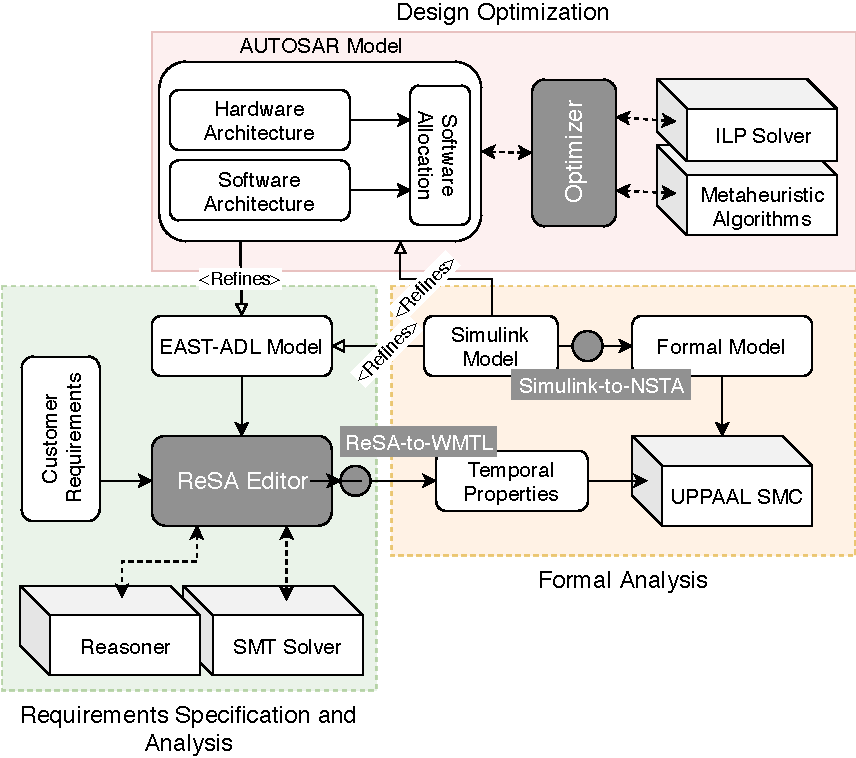
\includegraphics[width=\linewidth]{images/softdevflow}
        \else
        		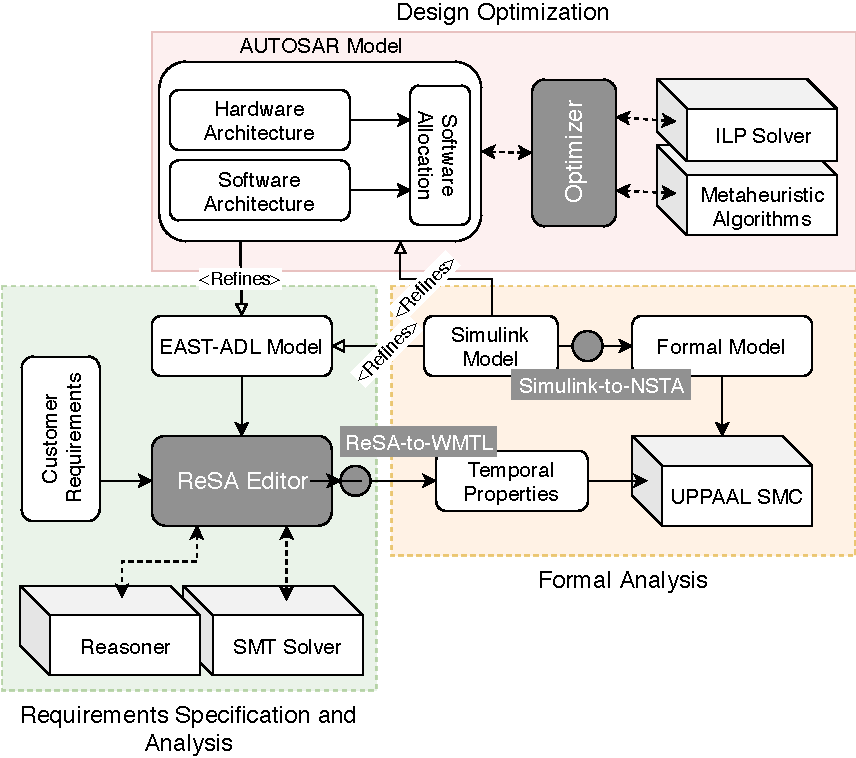
\includegraphics[width=1.0\linewidth]{images/softdevflow.eps}
		\fi
	\caption{Thesis Contributions Workflow.} 
    \end{figure}
\begin{itemize}
    \item \textbf{Formal Analysis of natural language requirements: } Most software and system requirements \cite{ieereqspecstandard} of embedded systems are specified in natural language, in fact it has become the de facto standard in industry, which is mainly because it is intuitive as opposed to computer languages, but also is expressive and flexible that many software engineers and other stakeholders find it easy to use. However, it is inherently ambiguous and therefore could lead to ambiguous and incomprehensible specifications. 
    As opposed to the use of templates \cite{Hull2011RequirementsEngineering}, specification patter systems\cite{Gruhn2006PatternsSpecifications,Konrad2005Real-timePatterns} , we propose a fairly expressive, flexible yet structured and domain domain-specific language, called \textit{ReSA} [ref] that utilizes the EAST-ADL architectural language to improve its effectiveness by reducing syntactic and semantic ambiguities of specifications. The language has translation in Boolean and description logic to support rigorous analysis using existing formal method tools, e.g., SMT solving, reasoners (inference engines) to detect, e.g., logical inconsistencies. Moreover, by translating interesting specifications to TCTL and WMTL properties, the language can be used to abstract syntactic complexity there by simplifying properties specification, e.g., for use in the model checking of Simulink model, after translation to formal model as briefly discussed  in the next contribution.
    \item \textbf{Scalable analysis of Simulink models: }
    Many safety-critical embedded systems are developed in Simulink \cite{JamesB.Dabney2003MasteringSimulink}, which is the de facto modeling language employed in industry.  To provide assurance that Simulink models fulfill given functional and timing requirements, we propose a pattern-based, execution-order preserving automatic transformation of atomic and composite Simulink blocks into stochastic timed automata that can be formally analyzed using UPPAAL Statistical Model Checker \cite{Bulychev2012UPPAAL-SMC:Automata}. Our method is scalable, and has been validated on industrial use cases \cite{Filipovikj2016SimulinkSystems}. The statistical model checker analyzes a state-transition system by conducting statistical analysis on the collected traces of the system executions, effectively mitigating the state-space explosion of (exact) model checking \cite{Legay2010StatisticalOverview}. 

    \item \textbf{Deployment optimization of distributed software applications: }
    At the system design level, the requirements specifications are realized by a system architecture of software and hardware parts that are constructed by functional components (or modules) that abstract the functionality of the system. In the platform-based development approach \cite{Sangiovanni-Vincentelli2004BenefitsDesign}, the system design should take into account consumption of critical hardware resources, such as power consumption, for two main reasons: optimizing power consumption is beneficial in order i) to accommodate more applications as well as to support power-intensive applications, and ii) to increase battery-life by lowering the amount of heat released by electronic components in the system. In this thesis, we propose an exact software allocation approach, as well as a heuristic one, for multirate systems that need to meet both timing and reliability.
    \item \textbf{Validation on industrial use cases: } 
    Our contributions such as its the ReSA language as well as the proposed formal analysis of Simulink model is validated on industrial use cases, which are provided
\end{itemize}

The rest of the thesis proposal is organized as follows. Section \ref{section:goals} introduces the research goals and the scientific contributions to address the research goals. Section \ref{section:methods} presents the research methods applied to conduct the research especially in the context of academic-industry collaboration. Section \ref{section:outline} shows the proposed outline of the thesis, followed by the presentation of the research progress in Section \ref{section:progress}, including the time plan until the doctoral defense. Section \ref{section:thirdcycle} presents the third-cycle outcomes, adapted from the individual study plan (ISP). Finally, Section \ref{section:related} discusses the related work before concluding the proposal in Section \ref{section:conclusions}.

\section{Thesis Outline Overview}
The thesis is divided into two parts. The first part is a summary of our research. It is organized as follows: in Chapter 2, we give the background information on requirements boilerplates, description logic, boolean satisfiability problem, Simulink, network of Stochastic Timed Automata. In Chapter 4, we describe the research problems and outline the research goals. In Chapter 3, we describe the research method employed to conduct the research. The thesis contribu- tions are described in Chapter 5, followed by the related work in Chapter 6. Finally, in Chapter 7, we conclude the thesis and outline possible directions for future work.
The second part is a collection of papers included in this thesis, listed as follows: